% WebGPU Geant4-DNA — arXiv preprint draft
% Build: pdflatex main && bibtex main && pdflatex main && pdflatex main
% NOTE: every quantitative value here is sourced from README.md § Numbers
% (the repo's single source of truth) and its committed JSON artifacts.
% Citations in refs.bib are flagged where bibliographic details still need
% verification before submission — see the banner in refs.bib.
\documentclass[11pt]{article}
\usepackage[utf8]{inputenc}
\usepackage[T1]{fontenc}
\usepackage{lmodern}
\usepackage[margin=1in]{geometry}
\usepackage{amsmath,amssymb}
\usepackage{booktabs}
\usepackage{graphicx}
\usepackage{siunitx}
\usepackage{xcolor}
\usepackage[hidelinks]{hyperref}
\usepackage{caption}
\usepackage{tikz}

% Placeholder for figures to be generated from the committed artifacts.
\newcommand{\placeholderfig}[2]{%
  \begin{center}\fbox{\parbox{0.92\linewidth}{\centering\vspace{1.2em}
  \textbf{[Figure placeholder: #1]}\\[0.4em]
  \footnotesize\itshape #2\vspace{1.2em}}}\end{center}}

\title{\textbf{WebGPU Geant4-DNA:} browser-native, kernel-fused\\
Monte Carlo track-structure simulation for radiobiology,\\
validated against Geant4 11.4.1}
\author{Ahmet Bar\i{}\c{s} G\"unayd\i{}n\\
\small Independent researcher \quad\textbar\quad \texttt{webgpudna.com}}
\date{\today}

\begin{document}
\maketitle

\begin{abstract}
We present a WebGPU/WGSL re-implementation of Geant4-DNA track-structure
physics and Karamitros Independent-Reaction-Time (IRT) radiolysis chemistry
that runs entirely in a web browser, with no CUDA toolchain and no
installation. The simulation uses a \emph{kernel-fusion} architecture: one
GPU thread per primary electron executes the full particle history inside a
single fused compute dispatch, eliminating per-step dispatch overhead. We do
not transpile Geant4; we re-implement its physics models from the Geant4-DNA
source and the G4EMLOW~8.8 tabulated cross sections, and use a
normally-compiled Geant4~11.4.1 as a validation oracle on a falsifiable,
artifact-backed ladder. Cross sections match the reference to peak ratios of
\numrange{0.975}{1.000}; the continuous-slowing-down range at \SI{10}{keV} is
\num{0.988}$\times$ Geant4. WebGPU track-structure tracking (Phases~A+B) runs
\textbf{455$\times$} faster than Geant4 single-thread (280$\times$ vs.\ an
8-thread build) on an Apple~M2~Pro, but we are explicit that this is
\emph{not} apple-to-apple: the Geant4 figure is whole-process wall-clock
(init, DNA physics-table construction, and per-event ntuple I/O included),
whereas the WGSL figure is dispatch-only, and the kernel-fusion architecture
itself accounts for only ${\sim}2\times$ of it (the fused Phase~A is 2\,\% of
the tracking time; Phase~B is an un-fused wavefront). The honest like-for-like
figure is the \emph{end-to-end} \textbf{1.48$\times$}, where both pipelines do
the same work and the IRT radiolysis chemistry on CPU dominates the
wall-clock---we report all of these and are explicit about which is which. We also report the project's honest limits: a 27\,\%
cascade-ionisation deficit traceable to an intentional excitation
cross-section choice, and the finding that the \emph{inter-track} chemistry
contribution---which closes most of the residual \SI{1}{\micro s} gap against
Geant4's \texttt{chem6}---is \emph{not} reachable browser-native, because
cross-primary IRT is $O(N^2)$ for a point source and GPU step-by-step
chemistry is bounded by the encounter radius to ${\sim}\num{50000}$ time
steps. These negative results are quantified and motivate a native runtime as
the path forward. All experiments are reproducible via committed JSON
artifacts.
\end{abstract}

\section{Introduction}
Geant4-DNA \cite{incerti2010geant4dna,bernal2015track,incerti2018geant4dna} is
the CNRS/IN2P3-coordinated extension of Geant4 \cite{agostinelli2003geant4}
for discrete, event-by-event Monte Carlo track-structure simulation in liquid
water at radiobiologically relevant (\si{eV}--\si{keV}) energies, together
with the subsequent radiolysis chemistry. It is the de-facto reference for
mechanistic modelling of radiation-induced DNA damage.

GPU acceleration of this class of simulation is an active area: gMicroMC
\cite{tsai2020gmicromc} and MPEXS-DNA \cite{okada2019mpexs} target
track-structure on the GPU, while GGEMS \cite{ggems} and GPUMCD
\cite{hissoiny2011gpumcd} target macroscopic dose. All of these are built on
CUDA or OpenCL and require a workstation-class install. To our knowledge there
is no open-source GPU Monte Carlo for radiation transport that runs
\emph{browser-native}---i.e.\ on the cross-vendor WebGPU API, with zero
install, on any machine with a modern browser. That accessibility gap is the
motivation here: a browser-native engine is trivially shareable, reproducible
without a toolchain, and usable for teaching and rapid validation.

Our contributions are: (i) a complete WebGPU/WGSL re-implementation of the
Geant4-DNA DNA\_Opt2 physics chain plus Karamitros IRT chemistry; (ii) a
kernel-fusion architecture that yields large speedups over single- and
multi-threaded Geant4; (iii) a research-grade, falsifiable validation ladder
against compiled Geant4~11.4.1, with every claim backed by a committed
artifact; and (iv) an honest characterisation of where the browser-native
approach reaches its limits, including a quantified negative result on the
inter-track chemistry contribution.

\section{Methods}

\subsection{Re-implementation, not transpilation}
None of Geant4's runtime executes on the GPU. Each physics model is
re-implemented as flat WGSL arithmetic, using the Geant4-DNA C++ source as the
algorithmic specification (sampling routines and formulae) and the
G4EMLOW~8.8 data files as the cross-section tables, converted once into WGSL
constant arrays. A normally-compiled Geant4~11.4.1 / G4EMLOW~8.8 install
serves as the \emph{validation oracle}: we run the \texttt{dnaphysics}
example single-threaded, dump its ntuples, and compare the WGSL output against
them---the same validate-against-compiled-Geant4 methodology used by
gMicroMC, MPEXS-DNA and GGEMS.

\subsection{Kernel-fusion architecture}
The pipeline has three phases (Fig.~\ref{fig:pipeline}):
\textbf{Phase~A (primaries)} is a single fused \texttt{@compute} dispatch with
one thread per primary electron; that thread runs the entire history---Born
ionisation, Emfietzoglou excitation, elastic and vibrational scattering---in a
\texttt{for} loop, with no per-step dispatch. \textbf{Phase~B (secondaries)}
is a wavefront stepper (one dispatch per physics step advancing all live
secondaries), which cannot be fused because the secondary count is unknown
until Phase~A completes. \textbf{Phase~C (chemistry)} runs the Karamitros
9-reaction IRT in a Web Worker off the main thread (a GPU spatial-hash
alternative exists but is less accurate at long times; see
Sec.~\ref{sec:intertrack}). Energy deposition into a $128^3$ voxel grid uses
fixed-point integer \texttt{atomicAdd} ($\times100$ per \si{eV}), since WGSL
atomics are integer-only.

\begin{figure}[t]
\centering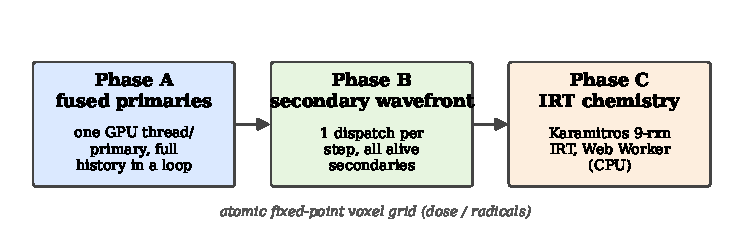
\includegraphics[width=0.92\linewidth]{figs/fig1_pipeline.pdf}
\caption{Three-phase pipeline. Phase~A is fully fused (one GPU thread per
primary, full history in a loop); B and C cannot be.}
\label{fig:pipeline}
\end{figure}

\subsection{Ported models and deliberate divergences}
We port Born ionisation (5 shells), Champion tabulated / screened-Rutherford
elastic, Sanche vibrational excitation (9 modes), and the Karamitros 9-reaction
IRT chemistry (6 species, Smoluchowski totally-diffusion-controlled and
Onsager-screened partially-diffusion-controlled types)
\cite{karamitros2011,karamitros2014}. Two deliberate departures from the
\texttt{DNA\_Opt2} defaults are documented (Table~\ref{tab:diverge}): we use
the Emfietzoglou excitation model \cite{emfietzoglou2005}---the model used by
the Geant4-DNA constructor \texttt{G4EmDNAPhysics\_option4}, which is unrelated
to the similarly-named EM~Standard list \texttt{G4EmStandardPhysics\_option4}---%
rather than Born, because it yields the correct
initial $G(\mathrm{H})=0.33$; and one tuning scalar,
\texttt{SIGMA\_EXC\_SCALE}$=0.5$, scaling the excitation cross section. A
second scalar present in the codebase, \texttt{RECOMB\_BOOST}, has no physical
basis; we measured it to be nearly inconsequential (Sec.~\ref{sec:discussion},
E10r) and set it to its neutral value $1.0$ for all reported chemistry, so the
$G$-values of \S\ref{sec:results} are parameter-free in that knob.

\begin{table}[t]\centering\footnotesize
\caption{Deliberate divergences from Geant4-DNA \texttt{DNA\_Opt2}, with the
measured cost of each (experiment IDs reference \S~Numbers).}
\label{tab:diverge}
\begin{tabular}{@{}llll@{}}
\toprule
Item & \texttt{DNA\_Opt2} & This work & Cost \\
\midrule
Excitation & Born & Emfietzoglou & $\sigma_{\text{exc}}$ $2.55\times$ (E6b) \\
$\sigma_{\text{exc}}$ scale & --- & $\times 0.5$ & net $1.27\times$ (E6c) \\
Recomb.\ boost & --- & off ($\times 1.0$) & $\Delta 1.4$\,pp RMS (E10r) \\
Chemistry pool & single & per-primary & $\Delta G(\mathrm{H_2})$ (E10f) \\
Dose reduction & fp64 & fp32 atomics & MC-equivalent, not bit-exact \\
\bottomrule
\end{tabular}
\end{table}

\subsection{WGSL constraints}
WGSL forbids recursion, dynamic dispatch and dynamic allocation, and allows
atomics only on \texttt{u32}. Consequently: all physics is inlined into
\texttt{main()}; secondaries are deferred to a buffer + wavefront rather than
recursed; dose uses fixed-point integers; and all memory is pre-allocated.

\subsection{Validation protocol}
The repository follows a six-level falsifiable ladder. Every experiment emits
a JSON artifact carrying the git SHA, a named seed, WGSL shader hashes, a pass
bar, and per-row observations; failed experiments are committed with
\texttt{status:"fail"} and a diagnosis rather than rerun. All numbers below
are drawn from this artifact set. The reference configuration is $N=4096$
primaries at \SI{10}{keV} on an Apple~M2~Pro (\texttt{apple/metal-3} adapter).
A reproducibility caveat applies: fp32 atomic reductions are not
order-deterministic across GPU vendors, so cross-hardware results are
statistically equivalent within Monte Carlo noise but not bit-exact.

\section{Results}
\label{sec:results}

\subsection{Cross sections (Level 1)}
All 9 cross-section channels match the G4EMLOW reference
(Table~\ref{tab:xs}). Sanche vibrational is bit-exact; the largest deviation
is the Champion elastic peak ratio at \num{0.975}.

\begin{table}[t]\centering\footnotesize
\caption{Cross-section validation vs.\ G4EMLOW 8.8. Peak ratio is
WebGPU/Geant4 at the worst single point; medians of the relative deviation
are $\sim\!10^{-3}$.}
\label{tab:xs}
\begin{tabular}{@{}llll@{}}
\toprule
Channel & Model & Peak ratio & Exp. \\
\midrule
Ionisation $\sigma_{\text{ion}}$ & Born (5 shells) & 0.9987 & E1 \\
Excitation $\sigma_{\text{exc}}$ & Emfietzoglou (5 lev.) & 0.9970 & E2 \\
Elastic $\sigma_{\text{el}}$ & Champion / scr.-Ruth. & 0.9751 & E3 \\
Vibrational $\sigma_{\text{vib}}$ & Sanche (9 modes) & 1.0000 & E4 \\
\bottomrule
\end{tabular}
\end{table}

\subsection{Track structure (Level 2)}
The continuous-slowing-down (CSDA) range at \SI{10}{keV} is \SI{2714.4}{nm}
vs.\ Geant4's \SI{2747.5}{nm}, i.e.\ $0.988\times$ ($3.59\sigma$), with energy
conservation at 100.0\,\% (E5). Across the eight ESTAR energies the deficit is
energy-dependent and was closed monotonically by the joint fix: the
\SI{100}{eV} ratio rose from $0.587\times$ to $0.736\times$ and all eight
energies improved, with the lift inversely proportional to the original
deficit---the expected signature of the excitation cross-section correction
(E5b, E5d; Fig.~\ref{fig:csda}).

\begin{figure}[t]
\centering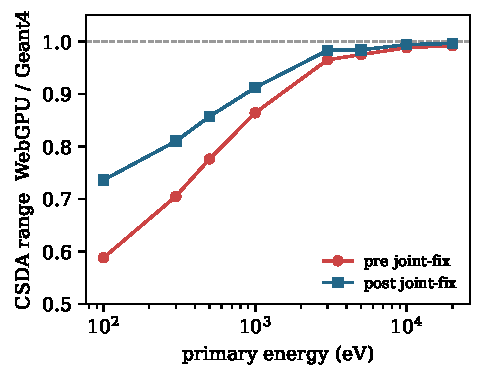
\includegraphics[width=0.6\linewidth]{figs/fig2_csda.pdf}
\caption{Energy-dependent CSDA closure under the joint fix: WebGPU/Geant4
range ratio at the eight ESTAR energies, pre vs.\ post fix (8/8 improved;
artifacts E5b, E5d).}
\label{fig:csda}
\end{figure}

The mean free path is 5--11\,\% short of Geant4 across six energy bins
(median $0.941$, E6). The full-cascade ionisation count is
\num{371.9} per primary vs.\ Geant4's \num{509.2}---a 27\,\% deficit at
$263\sigma$ (E7)---and the implicit $W$-value is \SI{26.89}{eV} vs.\ ICRU~31's
\SI{21.4}{eV} (\cite{icru31}, $+25.7\,\%$, E5c). Both are the same physics:
the intentional excitation inflation channels energy away from ionisation. The
secondary-electron kinetic-energy spectrum at creation matches to 1.0\,\%
overall, with 7/8 log-bins within 0.1--3.1\,\% (E8). Table~\ref{tab:track}
summarises.

\begin{table}[t]\centering\footnotesize
\caption{Track-structure metrics vs.\ Geant4 11.4.1 at \SI{10}{keV},
$N=4096$.}
\label{tab:track}
\begin{tabular}{@{}llll@{}}
\toprule
Metric & This work & Geant4 & Ratio (exp.) \\
\midrule
CSDA range & \SI{2714.4}{nm} & \SI{2747.5}{nm} & 0.988 (E5) \\
Energy cons. & 100.0\,\% & 99.99\,\% & 1.000 (E5) \\
Ions / primary & 371.9 & 509.2 & 0.730 (E7) \\
$W$-value & \SI{26.89}{eV} & \SI{21.4}{eV}$^\dagger$ & 1.257 (E5c) \\
Sec.\ KE/primary & 143.4 & 144.9 & 1.010 (E8) \\
\bottomrule
\end{tabular}
\\[0.3em]{\scriptsize $^\dagger$ ICRU 31 low-LET liquid water reference.}
\end{table}

\subsection{Chemistry (Levels 3--4)}
We report \emph{parameter-free} chemistry yields: the empirical
\texttt{RECOMB\_BOOST} knob (Table~\ref{tab:diverge}), which has no
first-principles basis, is set to its neutral value $1.0$. Against Geant4's
\texttt{chem6} at matched \SI{10}{keV}, the $G$-values at \SI{1}{\micro s}
(E10r) are then $G(\mathrm{OH})$ $0.91\times$, $G(\mathrm{e^-_{aq}})$
$0.86\times$, $G(\mathrm{H})$ $0.93\times$, $G(\mathrm{H_2})$ $0.74\times$,
$G(\mathrm{H_2O_2})$ $0.69\times$ (Fig.~\ref{fig:gvalues}), a five-species RMS
deviation of 19.7\,\% at \SI{1}{\micro s}.

Crucially, we measured that the knob is \emph{not} load-bearing: enabling it
($\times2.0$) changes the overall RMS deviation by only ${\sim}1.4$~pp (to
18.3\,\%), and although it lifts $G(\mathrm{H_2})$ it does so by introducing a
$1.10\times$ overshoot in $G(\mathrm{H})$ while leaving $G(\mathrm{H_2O_2})$
unchanged---so we drop it and report the parameter-free values above (E10r).
A first-principles replacement for its intended effect (super-excitation
autoionisation, or an Onsager/Mozumder escape-probability treatment of
geminate recombination) is left to future work (Sec.~\ref{sec:discussion}).

One result is energy-resolved and tuning-independent:
$G(\mathrm{e^-_{aq}})$ is non-monotonic between 1 and \SI{3}{keV}, a 12.5\,\%
dip significant at $126\sigma$ by primary-bootstrap
(Fig.~\ref{fig:vshape}, E10b), which \texttt{chem6} independently reproduces
(E10d)---real track-end / spur-structure physics, not an artifact.

\begin{figure}[t]
\centering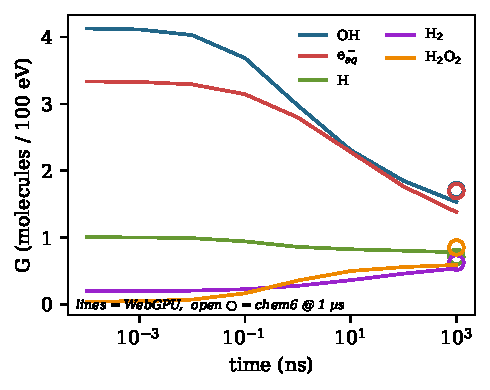
\includegraphics[width=0.62\linewidth]{figs/fig3_gvalues.pdf}
\caption{Radiolysis $G$-value time evolution---parameter-free WebGPU yields
(\texttt{RECOMB\_BOOST}~$=1.0$; lines) against Geant4 \texttt{chem6} endpoints
at \SI{1}{\micro s} (open circles). Artifact E10r.}
\label{fig:gvalues}
\end{figure}

\begin{figure}[t]
\centering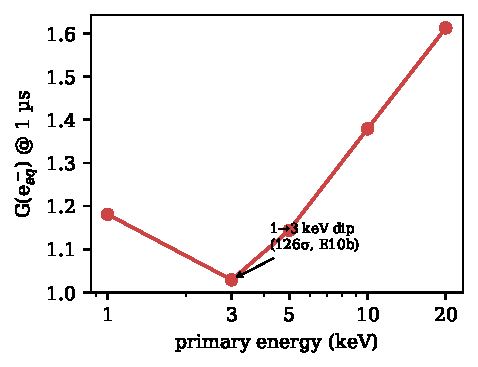
\includegraphics[width=0.58\linewidth]{figs/fig4_vshape.pdf}
\caption{$G(\mathrm{e^-_{aq}})$ at \SI{1}{\micro s} vs.\ primary energy: the
non-monotonic 1$\to$3~keV dip ($126\sigma$, E10b), independently reproduced by
\texttt{chem6} (E10d).}
\label{fig:vshape}
\end{figure}

\subsection{DNA damage (Level 5)}
We report Level~5 as a \emph{calibrated} damage model, not a validated
prediction, and state the distinction plainly. On a $21\times21$ B-DNA fibre
grid (\num{3.89}~Mbp target) the strand-break counts are the geometric
backbone-reach counts multiplied by per-event break probabilities:
$\mathrm{SSB_{dir}}=26=\lfloor 173\times P_{\mathrm{dir}}\rfloor$ with
$P_{\mathrm{dir}}=0.15$, and $\mathrm{SSB_{ind}}=64\approx 1423\times
P_{\mathrm{ind}}$ with $P_{\mathrm{ind}}=0.05$. The reported indirect/direct
ratio of 2.46 lies within PARTRAC's 2--3 band \cite{friedland2011}, but
$P_{\mathrm{ind}}$ was \emph{calibrated} (from the Geant4 default 0.4) to land
in that band; the ratio is therefore a fit, not an independent test, and
PARTRAC is itself a simulation.

Against experiment-calibrated cellular yields (\(\sim\)35~DSB and
\(\sim\)1000~SSB per diploid cell per Gy for low-LET radiation
\cite{ward1988}), the absolute per-Da yields are high by $223\times$ (SSB) and
$796\times$ (DSB) when normalised by the \emph{box-average} dose
(\SI{0.243}{Gy}). This is consistent in direction with track-core
concentration --- the fibre grid samples a $\sim$3~µm core in which the local
dose can plausibly reach tens of Gy --- but that concentration factor has not
been computed, so the absolute yields are presently neither validated nor
explained quantitatively. The outstanding terminal test (``E12-local'') is to
normalise yields by the \emph{local} dose the fibre grid actually receives,
read from the voxel dose grid, and check whether they collapse onto the
experimental per-Gy figures. Until that is done, Level~5 demonstrates that the
clustering kernel discriminates strand-break coincidences PARTRAC-like, not
that the code predicts absolute DNA-damage yields.

\subsection{Performance (Level 6)}
Phase~A+B tracking is \textbf{455$\times$} faster than Geant4~11.4.1
single-thread (\SI{635}{ms} vs.\ a \SI{289.1}{s} median over 3 trials, E15b)
and \textbf{280$\times$} vs.\ an 8-thread build (\SI{178.0}{s}, E15c). Peak
Phase~A throughput is \num{538947} primaries/s at $N=16384$ (E15). We state
three caveats so these numbers are not over-read. \emph{First, the comparison
is not apple-to-apple}: the Geant4 wall-clock is whole-process (process init,
DNA physics-table construction, the event loop, and per-event ntuple I/O all
included), while the WGSL \SI{635}{ms} is dispatch-only. \emph{Second, that
overhead is large}: Geant4 MT-8 scales only $1.62\times$ over single-thread
(not $8\times$), implying a substantial fixed/serial fraction --- a two-point
Amdahl read places ${\sim}\SI{160}{s}$ of the \SI{289}{s} in serial overhead,
so the pure-tracking speedup is materially below $455\times$ (we estimate
${\sim}200\times$; a like-for-like event-loop-only re-measurement, E15-fair,
is queued). \emph{Third, kernel fusion is not what delivers the large factor}:
a within-WebGPU comparison of the fused kernel against a modelled per-step
dispatch gives a \textbf{40$\times$} factor \emph{for Phase~A} (E16), but
Phase~A is only \SI{14.4}{ms} (2\,\%) of the \SI{635}{ms}; Phase~B is an
un-fused 2000-dispatch wavefront. Fusion's contribution to the full tracking
pipeline is therefore ${\sim}2\times$ (\SI{1324}{ms} naive $\to$
\SI{635}{ms} fused), with GPU data-parallelism over $N$ primaries supplying
the rest. The single honest like-for-like number is the \emph{end-to-end}
$1.48\times$, where both pipelines do the same work and the IRT chemistry on
CPU dominates the wall-clock (\SI{194}{s} of \SI{194.6}{s}); this motivates
Sec.~\ref{sec:intertrack}.

\begin{figure}[t]
\centering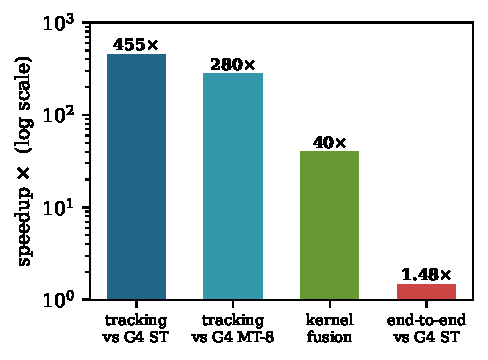
\includegraphics[width=0.58\linewidth]{figs/fig6_perf.pdf}
\caption{Speedups (log scale): fused track-structure kernel vs.\ Geant4
single-thread (E15b) and 8-thread (E15c), the within-WebGPU kernel-fusion
factor (E16), and the honest \emph{end-to-end} figure (E15b), which is only
$1.48\times$ because the IRT chemistry runs on CPU.}
\label{fig:perf}
\end{figure}

\section{The inter-track chemistry limitation}
\label{sec:intertrack}
The largest remaining gap vs.\ \texttt{chem6} is an \emph{inter-track} effect:
per-primary IRT partitioning misses cross-primary reactions that, when
included, add $\Delta G(\mathrm{H_2})=+0.149$ at \SI{1}{\micro s}---96\,\% of
the residual implementation gap (E10f). We asked whether this is recoverable
browser-native, and found it is not, by two independent routes.

\textbf{Cross-primary IRT is $O(N^2)$ for a point source.} The IRT reaction
horizon is the diffusion length over the full \SI{1}{\micro s} window,
$R_{\text{cut}}=1.45+2\sqrt{8 D_{\max} t_{\max}}\approx\SI{551}{nm}$, not the
few-nm contact scale. At \SI{10}{keV} the radicals occupy a ${\sim}\SI{5}{\micro m}$
blob, so a \SI{551}{nm} spatial hash spans most of it and prunes almost
nothing; over 50\,\% of accepted cross-primary reactions involve pairs more
than \SI{100}{nm} apart (E10k). The single-pool scan is ${\sim}10^{12}$
reaction-time samples (${\sim}70$ hr in-browser) and the heap is ${\sim}\SI{2}{GB}$.

\textbf{GPU step-by-step (SBS) chemistry is encounter-radius-bounded.} The
GPU radiolysis codes use a step-by-step Brownian-motion model in which a
reaction fires when two reactants fall within a Smoluchowski reaction radius
(gMicroMC \cite{tsai2020gmicromc}; MPEXS-DNA adds a during-step reaction
probability at small time steps \cite{okada2019mpexs}). We implemented this in
WGSL and, as a refinement, a Green's-function (Brownian-bridge) during-step
reaction probability \cite{clifford1986} from the step-by-step
radiation-chemistry literature, and measured its convergence against the
analytic Smoluchowski value for a single pair. The per-step cost is ${\sim}\SI{110}{ms}$ at $N=4096$ (E10L), and
the IRT-parity budget is ${\sim}1750$ steps. But accuracy requires a time step
that resolves the encounter radius $\sigma$, $\Delta t \lesssim
\sigma^2/(2D)\approx\SI{0.02}{ns}$, \emph{independent of pair separation or
density} (E10Q; Fig.~\ref{fig:killcrit})---so ${\sim}\num{50000}$ steps are
needed regardless. Compaction lowers per-step cost but not step count (E10P).
No SBS schedule, full or hybrid, beats the IRT worker at the required accuracy
on laptop WebGPU.

\begin{figure}[t]
\centering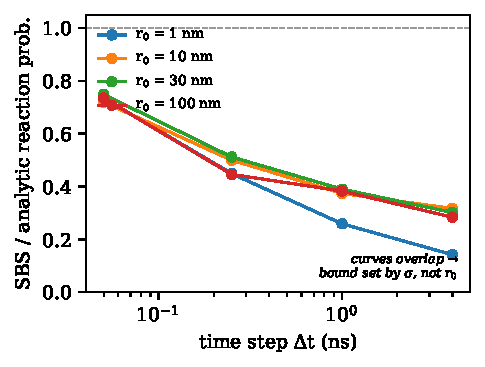
\includegraphics[width=0.6\linewidth]{figs/fig5_killcrit.pdf}
\caption{Kill criterion (E10Q): single-pair SBS/analytic reaction-probability
ratio vs.\ $\Delta t$ for four separations. The curves overlap, so the
$\Delta t$ requirement is set by the encounter radius $\sigma$, not by
separation — far, dilute pairs need the same tiny steps as close ones.}
\label{fig:killcrit}
\end{figure}

Both routes converge on the same conclusion: the inter-track physics requires
a \emph{native} runtime (e.g.\ Node/Deno + \texttt{wgpu-native}), where RAM is
cheap (unblocking single-pool cross-primary IRT) or many cores parallelise the
step count. The browser remains the validation and demonstration surface.

\section{Discussion}
\label{sec:discussion}
Browser-native execution buys accessibility and reproducibility that the
CUDA/OpenCL engines cannot: the simulation and its validation harness run on
any modern GPU with no install, which is valuable for teaching, sharing, and
independent re-checking of every artifact. The cost is the WebGPU feature
envelope (integer-only atomics, no recursion) and---per
Sec.~\ref{sec:intertrack}---an inter-track chemistry ceiling that pushes the
last increment of fidelity off-browser. The cascade-ionisation deficit and the
\texttt{RECOMB\_BOOST} fudge are open items with identified, falsifiable next
steps (super-excitation autoionisation; an Onsager escape-probability
treatment to replace the fudge). Relative to the CUDA codes gMicroMC and
MPEXS-DNA, our speedups come from
kernel fusion on a single consumer GPU (MPEXS-DNA, for reference, reports up
to 2900$\times$ over single-core Geant4-DNA on an NVIDIA TITAN~V
\cite{okada2019mpexs}); extending the same methodology to the
EM~Standard list \texttt{G4EmStandardPhysics\_option4} for macroscopic photon
dose is a natural, if substantially larger, direction.

\section{Conclusion}
A browser-native, kernel-fused WebGPU re-implementation reproduces Geant4-DNA
track structure to within a fraction of a percent on cross sections and
$0.988\times$ on CSDA range, at 455$\times$/280$\times$ the speed of
single-/multi-threaded Geant4, with an honest, artifact-backed account of its
limits---most notably the quantified result that the inter-track chemistry
contribution is not browser-native and requires a native runtime.

\section*{Data and code availability}
Source, the full validation ladder, and every JSON artifact are at
\url{https://github.com/abgnydn/webgpu-dna}; a live build runs at
\url{https://webgpudna.com}. A versioned Zenodo deposit accompanies release
\texttt{v0.4.0} (DOI to be inserted). Each experiment reruns via
\texttt{npm run experiments -- <id>}.

\bibliographystyle{plain}
\bibliography{refs}
\end{document}
